\section{Training}

X-Spanformer is trained end-to-end to jointly learn both span induction and controller fusion.  Denote by 
\(\mathcal{D}=\{(x^{(i)},y^{(i)})\}_{i=1}^N\) 
the training corpus, where each input \(x^{(i)}\) is a sequence of \(T\) Unicode codepoints encoded into seed embeddings \(H^0\in\mathbb{R}^{T\times d}\) (Section 3.1).  Let \(H=\mathrm{Encoder}(H^0)\in\mathbb{R}^{T\times d}\) be the contextualized representations.  The model optimizes a composite loss

\[
\mathcal{L}_{\mathrm{total}}
= \mathcal{L}_{\mathrm{task}}
+ \beta_1\,\mathcal{L}_{\mathrm{span}}
+ \beta_2\,\mathcal{L}_{\mathrm{ent}},
\]

where
\(\mathcal{L}_{\mathrm{task}}\) is a task‐specific objective (e.g.\ cross‐entropy or contrastive loss),
\(\mathcal{L}_{\mathrm{span}}\) encourages alignment to any available span supervision, and
\(\mathcal{L}_{\mathrm{ent}}\) is an entropy‐based regularizer that drives early exploration.

The training pipeline consists of three fully differentiable stages:
\begin{itemize}
	\item \textbf{Span induction with entropy‐regularized scoring}: generate and score candidate spans via a differentiable pointer network (Section 3.2), regularized to maintain high entropy early on.
	\item \textbf{Relevance‐weighted fusion}: pool and encode the top-\(K\) spans, compute relevance logits, and interpolate into a controller vector \(s\) (Section 3.5–3.7).
	\item \textbf{Controller‐aware injection}: condition the transformer backbone via prefix insertion, attention‐bias shifts, or gated FFN (Section 3.6).
\end{itemize}

\subsection{Span Induction with Entropic Regularization}
\label{sec:span-induction}

Starting from contextualized embeddings \(H\in\mathbb{R}^{T\times d}\), we define the set of contiguous spans of maximum width \(w_{\max}\):
\begin{equation}
	S = \bigl\{(i,j)\;\big|\;1\le i<j\le \min(i+w_{\max},T)\bigr\}.
	\label{eq:contiguous_span_set}
\end{equation}
Each span \((i,j)\in S\) is pooled to a fixed-length vector
\[
v_{ij} = \mathrm{Pool}\bigl(H[i:j]\bigr)\in\mathbb{R}^d,
\]
and scored by a small induction network \(f_{\mathrm{ind}}:\mathbb{R}^d\to\mathbb{R}\):
\[
w_{ij} = f_{\mathrm{ind}}(v_{ij}).
\]
We normalize these logits to obtain a distribution over spans:
\begin{equation}
	P_{ij}
	= \frac{\exp(w_{ij})}
	{\sum_{(a,b)\in S}\exp(w_{ab})}.
	\label{eq:span_softmax}
\end{equation}

To prevent early collapse into a few high–confidence spans, we add a temperature–weighted entropy penalty:
\begin{equation}
	\mathcal{L}_{\mathrm{ent}}
	= -\lambda_{\mathrm{ent}}(t)\;H(P),
	\quad
	H(P) = -\sum_{(i,j)\in S}P_{ij}\log P_{ij},
	\label{eq:entropy_term}
\end{equation}
with an annealing schedule
\begin{equation}
	\lambda_{\mathrm{ent}}(t)
	= \lambda_0\,e^{-\gamma t},
	\label{eq:entropy_decay}
\end{equation}
where \(t\) indexes training epochs, \(\lambda_0>0\) is the initial weight\footnote{We set $\lambda_0 = 1.0$ to ensure equal weighting between span entropy and task loss during initial exploration phases.}, and \(\gamma>0\) the decay rate\footnote{Decay rate $\gamma = 0.1$ provides gradual sparsification over 50 epochs, balancing exploration with convergence to interpretable spans.}.  This follows entropy regularization principles \cite{grandvalet2005semi,pereyra2017regularizing} and curriculum learning schedules \cite{bengio2009curriculum,kreutzer2021distilling}.

\begin{proposition}[Maximum Entropy of Uniform Span Distribution]
	\label{prop:span_entropy_bound}
	Let \(|S|=N\).  Then the entropy \(H(P)\) in Equation~\eqref{eq:entropy_term} is maximized when
	\begin{equation}
		P_{ij} = \frac{1}{N}
		\quad\forall\,(i,j)\in S,
		\label{eq:uniform_P}
	\end{equation}
	yielding
	\begin{equation}
		H_{\max}(P) = \log N.
		\label{eq:max_entropy}
	\end{equation}
\end{proposition}
\begin{proof}
	We maximize the entropy function
	\[
	H(P) = -\sum_{(i,j)\in S} P_{ij} \log P_{ij}
	\]
	subject to the normalization constraint \(\sum_{(i,j)\in S} P_{ij} = 1\) and non-negativity \(P_{ij} \geq 0\).
	
	\textbf{Step 1:} Construct the Lagrangian functional.
	\[
	\mathcal{L}(P, \lambda) = -\sum_{(i,j)\in S} P_{ij} \log P_{ij} + \lambda\left(\sum_{(i,j)\in S} P_{ij} - 1\right)
	\]
	
	\textbf{Step 2:} Compute the first-order optimality condition for \(P_{kl}\) where \((k,l) \in S\).
	\[
	\frac{\partial \mathcal{L}}{\partial P_{kl}} = -\log P_{kl} - 1 + \lambda = 0
	\]
	
	\textbf{Step 3:} Solve for \(P_{kl}\).
	\[
	\log P_{kl} = \lambda - 1 \quad \Rightarrow \quad P_{kl} = e^{\lambda - 1}
	\]
	
	\textbf{Step 4:} Since this relation holds for every \((k,l) \in S\), all probabilities are equal: \(P_{ij} = c\) for some constant \(c = e^{\lambda - 1}\).
	
	\textbf{Step 5:} Apply the normalization constraint.
	\[
	\sum_{(i,j)\in S} P_{ij} = \sum_{(i,j)\in S} c = |S| \cdot c = N \cdot c = 1
	\]
	Therefore, \(c = \frac{1}{N}\), which gives \(P_{ij} = \frac{1}{N}\) for all \((i,j) \in S\).
	
	\textbf{Step 6:} Substitute into the entropy expression.
	\[
	H_{\max}(P) = -\sum_{(i,j)\in S} \frac{1}{N} \log\left(\frac{1}{N}\right) = -\frac{N}{N} \log\left(\frac{1}{N}\right) = -\log\left(\frac{1}{N}\right) = \log N
	\]
\end{proof}

\noindent\textbf{Remark.} Early in training, a high \(\lambda_{\mathrm{ent}}(t)\) encourages broad span exploration.  As \(\lambda_{\mathrm{ent}}(t)\) decays, the model concentrates probability mass on a sparse set of high‐salience spans, facilitating convergence to meaningful structural units.

\subsection{Controller-Aware Generation and Final Objective}
\label{sec:controller-injection}

The fused controller vector 
\(\displaystyle \tilde{s} = \sum_{k=1}^K a_k\,s_k\in\mathbb{R}^d\) 
(where \(a_k=\exp(w_k)/\sum_{m}\exp(w_m)\) and \(w_k=g_\phi(s_k,\delta_k,c_k)\)) serves as a global conditioning signal for the transformer encoder.  X-Spanformer supports three fully differentiable injection pathways that bias computation at different stages of the network (Figure~\ref{fig:controller_injection_modes}).

\begin{figure}[H]
	\centering
	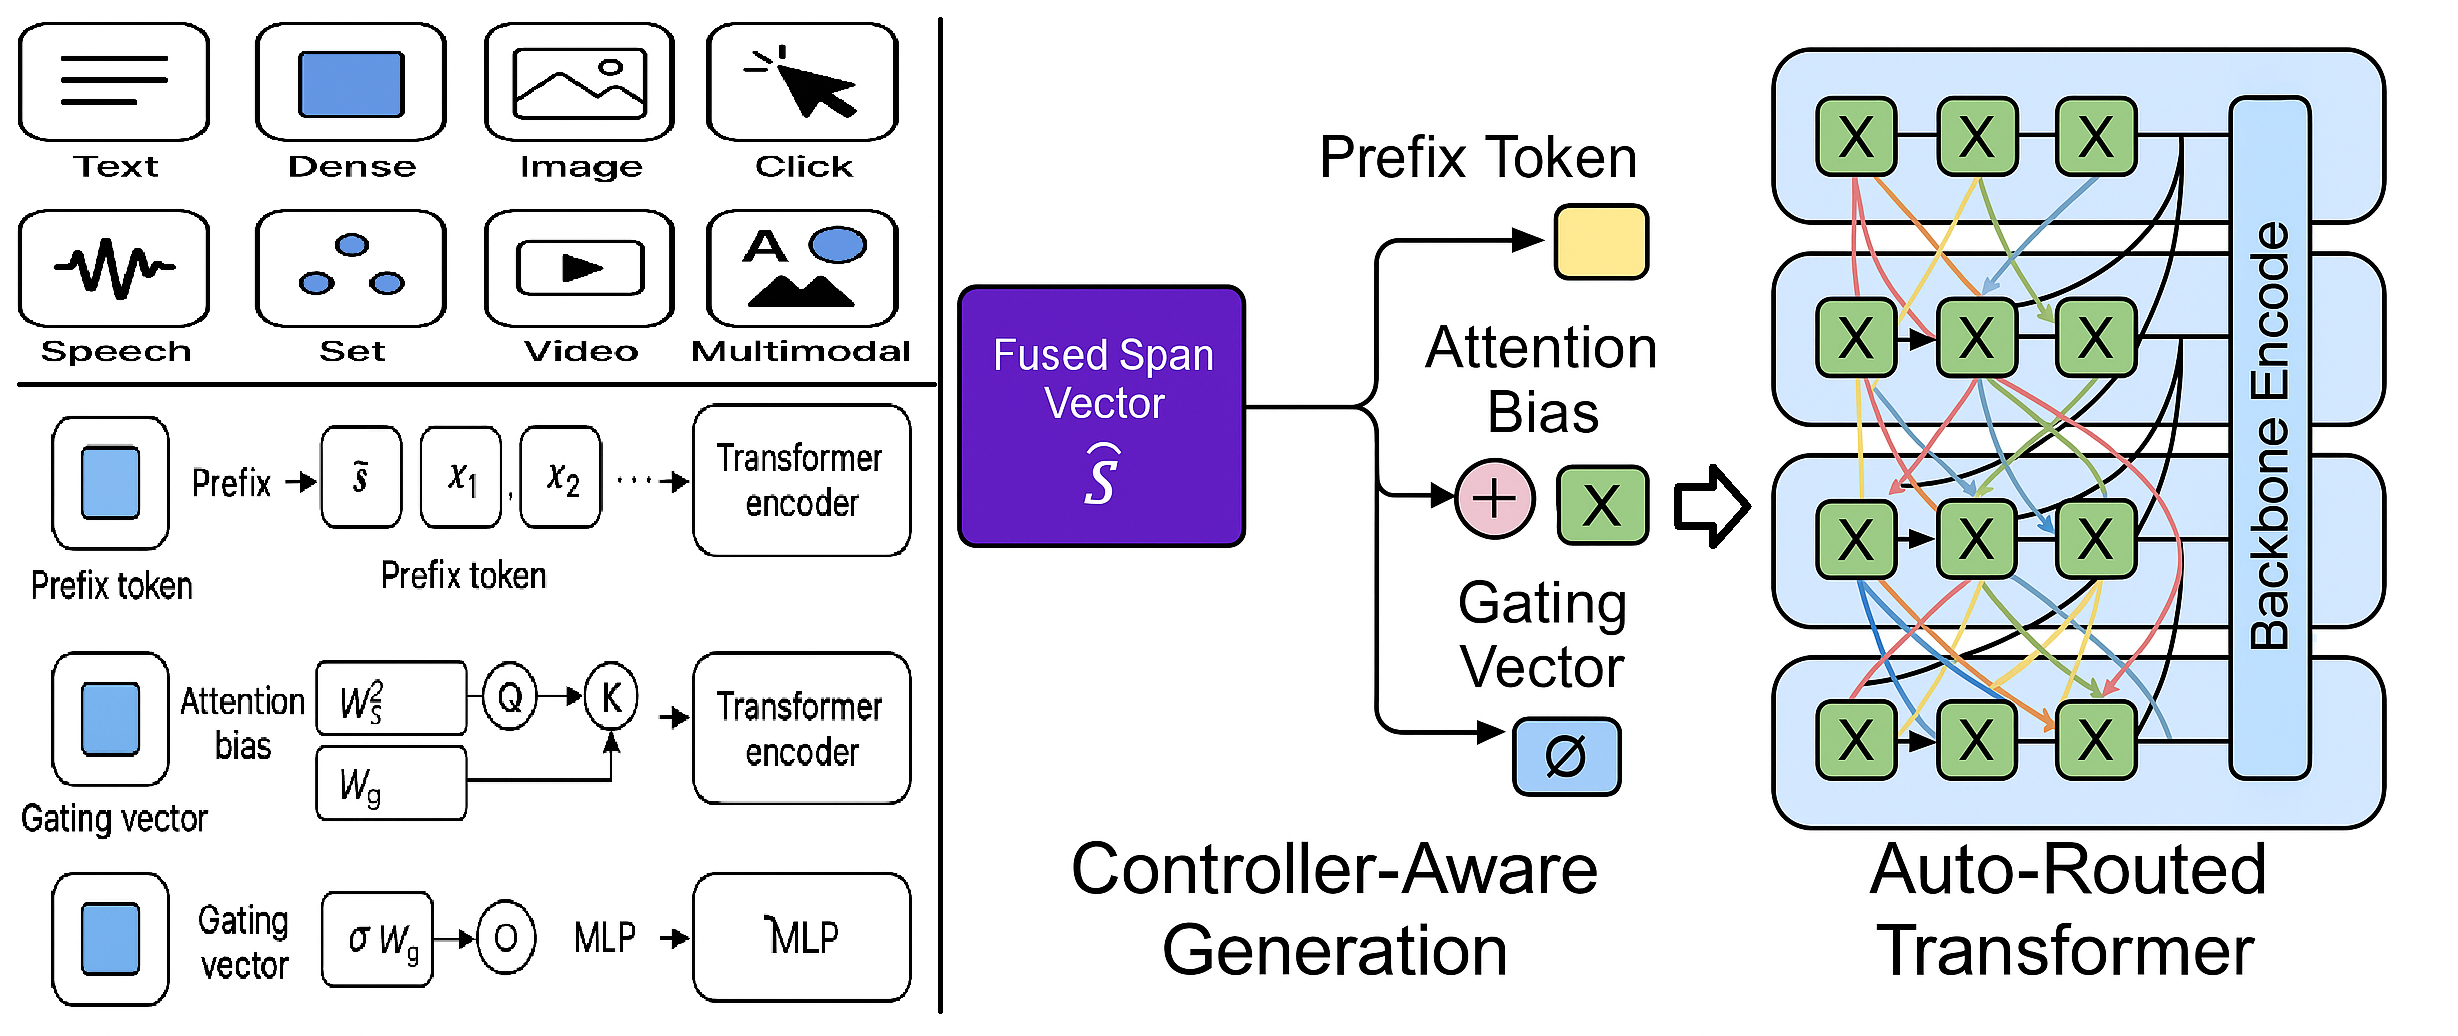
\includegraphics[width=0.92\textwidth]{figures/figure_5.png}
	\caption{Controller injection modes: prefix-token insertion, attention-bias adaptation, and gated FFN modulation.}
	\label{fig:controller_injection_modes}
\end{figure}

\subsubsection{Prefix-Token Injection}
We prepend \(\tilde{s}\) as a synthetic token at position 0:
\[
H' = \bigl[\tilde{s};\,h_1;\dots;h_T\bigr]\in\mathbb{R}^{(T+1)\times d}.
\]
A learned position embedding for index 0 ensures \(\tilde{s}\) participates in all attention heads from the first layer \cite{li2021prefix}. 

\subsubsection{Attention-Bias Injection}
We modify the attention logits by adding low-rank biases derived from \(\tilde{s}\):
\[
Q_i \;\leftarrow\; Q_i + W_Q\,\tilde{s},
\quad
K_j \;\leftarrow\; K_j + W_K\,\tilde{s},
\]
so that attention scores become 
\(\exp\bigl((Q_i + W_Q\tilde{s})^\top(K_j + W_K\tilde{s})\bigr)\).  
Here \(W_Q,W_K\in\mathbb{R}^{d\times d}\) learn to steer query and key subspaces \cite{hu2021lora}.  

\subsubsection{Gated-FFN Injection}
At each transformer layer, we modulate the feed-forward output by a span-conditioned gate:
\[
g = \sigma\bigl(W_g\,\tilde{s} + b_g\bigr)\in(0,1)^d,
\quad
h_i' = h_i + g \odot \mathrm{FFN}(h_i),
\]
where \(W_g\in\mathbb{R}^{d\times d}\), \(\sigma\) is sigmoid, and \(\odot\) denotes elementwise multiplication.  This gate adaptively amplifies or attenuates nonlinear transformations based on span context \cite{shazeer2017outrageously}.

\subsubsection{Semantic Routing Interpretation}
Injecting \(\tilde{s}\) as a dynamic, learned prompt parallels latent prompting and adapter routing frameworks (e.g.\ \cite{raffel2020exploring,liu2022pada,gupta2022molt}).  Unlike fixed metadata tags, our controller emerges from differentiable span selection, yielding semantically grounded routing signals.

\subsubsection{End-to-End Differentiability}
\begin{proposition}
	\label{prop:controller_diff}
	If each span embedding \(s_k=\mathrm{Pool}(x_{i_k:j_k})\) is a differentiable function of \(x\), and \(\tilde{s}\) is computed by
	\(\tilde{s}=\sum_k a_k s_k\) with \(a_k=\softmax(w_k)\), then for all three injection modes—prefix, bias, and gated-FFN—the final task loss \(\mathcal{L}\) is differentiable with respect to the span scorer parameters, pooling operator, and encoder parameters.
\end{proposition}
\begin{proof}
	We establish differentiability by showing that each injection mode creates a differentiable path from input \(x\) to task loss \(\mathcal{L}\).
	
	\textbf{Given assumptions:}
	\begin{enumerate}
		\item Each span embedding \(s_k = \mathrm{Pool}(x_{i_k:j_k})\) is differentiable in \(x\)
		\item Controller weights \(a_k = \softmax(w_k)\) where \(w_k\) are learnable parameters
		\item Fused controller \(\tilde{s} = \sum_{k=1}^K a_k s_k\)
	\end{enumerate}
	
	\textbf{Step 1:} Show \(\tilde{s}\) is differentiable in \(x\).
	Since \(s_k\) is differentiable in \(x\) by assumption, and \(a_k = \softmax(w_k)\) is differentiable in \(w_k\), we have:
	\[
	\frac{\partial \tilde{s}}{\partial x} = \sum_{k=1}^K a_k \frac{\partial s_k}{\partial x} + \sum_{k=1}^K s_k \frac{\partial a_k}{\partial w_k} \frac{\partial w_k}{\partial x}
	\]
	Both terms exist by the chain rule and differentiability assumptions.
	
	\textbf{Step 2:} Analyze each injection mode.
	
	\textit{Case 1 - Prefix injection:} \(H' = [\tilde{s}; h_1; \ldots; h_T]\)
	The augmented sequence passes through standard transformer attention:
	\[
	\frac{\partial \mathcal{L}}{\partial \tilde{s}} = \frac{\partial \mathcal{L}}{\partial H'} \frac{\partial H'}{\partial \tilde{s}}
	\]
	Since \(\frac{\partial H'}{\partial \tilde{s}} = [1; 0; \ldots; 0]\), gradients flow directly to \(\tilde{s}\).
	
	\textit{Case 2 - Attention bias:} \(Q_i \leftarrow Q_i + W_Q \tilde{s}\), \(K_j \leftarrow K_j + W_K \tilde{s}\)
	Attention scores become \(A_{ij} = \exp((Q_i + W_Q \tilde{s})^T(K_j + W_K \tilde{s}))\).
	\[
	\frac{\partial A_{ij}}{\partial \tilde{s}} = A_{ij} \left[ (K_j + W_K \tilde{s})^T W_Q + (Q_i + W_Q \tilde{s})^T W_K \right]
	\]
	This is well-defined since exponential and linear functions are differentiable.
	
	\textit{Case 3 - Gated FFN:} \(h_i' = h_i + g \odot \mathrm{FFN}(h_i)\) where \(g = \sigma(W_g \tilde{s} + b_g)\)
	\[
	\frac{\partial h_i'}{\partial \tilde{s}} = \frac{\partial g}{\partial \tilde{s}} \odot \mathrm{FFN}(h_i) = \sigma'(W_g \tilde{s} + b_g) \odot W_g \odot \mathrm{FFN}(h_i)
	\]
	Since \(\sigma\) is the sigmoid function, \(\sigma'\) exists everywhere.
	
	\textbf{Step 3:} Apply chain rule.
	In all cases, \(\frac{\partial \mathcal{L}}{\partial x} = \frac{\partial \mathcal{L}}{\partial \tilde{s}} \frac{\partial \tilde{s}}{\partial x}\) exists by composition of differentiable functions.
\end{proof}

\subsubsection{Final Objective}
Let \(\mathcal{L}_{\mathrm{task}}\) be the downstream loss (e.g.\ cross-entropy or contrastive).  The total training objective is
\[
\mathcal{L}
= \mathcal{L}_{\mathrm{task}}
+ \beta_1\,\mathcal{L}_{\mathrm{span}}
+ \beta_2\,\mathcal{L}_{\mathrm{ent}},
\]
where \(\beta_1,\beta_2\ge0\) balance structural supervision and entropy regularization.\footnote{Typical ranges: \(\beta_1\in[0.5,1.5]\), \(\beta_2<0.3\) after warmup for stable sparsity.}

\subsection{End-to-End Fine-Tuning}
\label{sec:end-to-end-finetuning}

After the span scorer \(f_\theta\) and aggregator \(g_\phi\) have learned stable inductive patterns, we integrate the fused controller \(\tilde{s}\) into the transformer backbone \(\psi\) and optimize all components jointly.

\subsubsection{Joint Routing and Regularization}
\label{sec:joint-routing-regularization}

The total objective over epochs \(t=T_1+1,\dots,T_2\) is

\begin{equation}
	\mathcal{L}_{\mathrm{total}}(t)
	= \mathcal{L}_{\mathrm{task}}
	+ \beta_{1}\,\mathcal{L}_{\mathrm{span}}
	+ \beta_{2}\,\lambda_{\mathrm{ent}}(t)\,H(P),
	\label{eq:curriculum_total}
\end{equation}

where
\(\mathcal{L}_{\mathrm{task}}\) is the downstream loss (e.g., negative log‐likelihood, classification cross‐entropy, or contrastive objective),  
\(\mathcal{L}_{\mathrm{span}} = \mathrm{KL}\bigl(P_{\mathrm{gold}}\Vert P_{\theta}\bigr)\) aligns the induced span distribution \(P_\theta\) with any available span supervision, and  
\(H(P)\) is the Shannon entropy of \(P_\theta\).  
The entropy coefficient is annealed only after the Phase I transition epoch \(T_1\):
\begin{equation}
\lambda_{\mathrm{ent}}(t)
= \lambda_{0}\,\exp\bigl(-\gamma\,(t - T_1)\bigr)\,\mathbf{1}_{t > T_1},
\label{eq:entropy_schedule}
\end{equation}
ensuring continued but diminishing exploration during fine‐tuning.

\textbf{Mathematical Properties of the Annealing Schedule:}
\begin{enumerate}[leftmargin=1.5em]
\item \emph{Continuity at Transition:} \(\lim_{t \to T_1^+} \lambda_{\mathrm{ent}}(t) = \lambda_0\)
\item \emph{Monotonic Decay:} For \(t > T_1\), \(\frac{d\lambda_{\mathrm{ent}}}{dt} = -\gamma \lambda_0 \exp(-\gamma(t-T_1)) < 0\)
\item \emph{Asymptotic Behavior:} \(\lim_{t \to \infty} \lambda_{\mathrm{ent}}(t) = 0\)
\end{enumerate}
This exponential decay balances initial exploration (\(\lambda_0\)) with eventual exploitation (convergence to 0).

\subsubsection{Training Algorithm}
\label{sec:training-algorithm}

\medskip
\noindent\textbf{Algorithm: Joint Optimization}

\begin{algorithm}[H]
	\caption{End‐to‐End Fine‐Tuning}
	\label{alg:e2e_finetuning}
	\begin{algorithmic}[1]
		\REQUIRE Pretrained scorer \(f_\theta\), aggregator \(g_\phi\), transformer \(\psi\)
		\FOR{epoch \(t=T_1+1\) to \(T_2\)}
		\FOR{each batch \((x,y)\)}
		\STATE Compute contextual embeddings \(H = \psi_{\mathrm{enc}}(x)\)
		\STATE Enumerate spans \(S\) and pool \(v_{ij} = \mathrm{Pool}(H[i:j])\)
		\STATE Induce span logits \(w_{ij}=f_\theta(v_{ij})\), normalize 
		\(P_{ij}=\softmax(w)\)
		\STATE Select top-\(K\) spans \(\{s_k\}\) and compute \(\tilde{s}=\sum_k a_k s_k\)
		\STATE Inject \(\tilde{s}\) into \(\psi\) via prefix/bias/gate
		\STATE Compute \(\mathcal{L}_{\mathrm{total}}(t)\) by Eq.~\eqref{eq:curriculum_total}
		\STATE Backpropagate and update \(\theta,\phi,\psi\)
		\ENDFOR
		\ENDFOR
	\end{algorithmic}
\end{algorithm}

\noindent\textbf{Summary.} This joint training approach combines span induction (\(f_\theta\)), aggregation (\(g_\phi\)), and the transformer parameters \(\psi\), using the controller vector \(\tilde{s}\) as a structural bottleneck.  This combined optimization:
\begin{itemize}
	\item Preserves high‐entropy exploration early in fine‐tuning,  
	\item Gradually shifts focus to task‐relevant spans via entropy annealing,  
	\item Learns to route structural information into the encoder through differentiable injection modes.
\end{itemize}
Empirically, this two‐stage curriculum yields stable convergence under sparse span supervision and enhances interpretability of transformer behavior \cite{belinkov2022probing}.

\subsubsection{Optimization Details}
\label{sec:optimization-details}

\medskip
\noindent We train all parameters with AdamW \cite{loshchilov2019decoupled}, using:
\begin{itemize}[leftmargin=1.5em]
	\item Cosine learning‐rate schedule with 10\% warmup,
	\item Gradient clipping at \(\|\nabla\|_2\le1.0\),
	\item Dropout rate 0.1,
	\item Batch size 64 (token‐aligned).
\end{itemize}
Full hyperparameter ranges and ablation settings are provided in Appendix~\ref{sec:hyperparams} and \ref{sec:ablation-settings}.
